\documentclass[preprint,12pt]{elsarticle}
\usepackage{lineno,hyperref}
\usepackage{booktabs}
\usepackage[english]{babel}
\usepackage[utf8]{inputenc}
\usepackage{amsfonts}
\usepackage{graphicx}
\usepackage{amssymb,amsmath}
\usepackage{float}
\usepackage{ragged2e}
\usepackage{adjustbox}
\usepackage{multicol}
\usepackage{mwe}
\usepackage[justification=centering]{caption}

\usepackage{algorithm}
\usepackage{algpseudocode}

\usepackage{multirow}
\usepackage{mathtools}
\usepackage{color}
\usepackage{soul}
\usepackage{comment}
\usepackage{lscape}
\usepackage{setspace}
\doublespacing

\algnewcommand\algorithmicforeach{\textbf{for each}}
\algdef{S}[FOR]{ForEach}[1]{\algorithmicforeach\ #1\ \algorithmicdo}

\newcommand\tab[1][0.73cm]{\hspace*{#1}}

\usepackage{tikz}
\usetikzlibrary{arrows.meta,positioning,calc}
\usepackage{pgfplots}
\pgfplotsset{compat=1.17}
\def\checkmark{\tikz\fill[scale=0.3](0,.35) -- (.25,0) -- (1,.7) -- (.25,.15) -- cycle;}

\usepackage{array}
\newcolumntype{L}[1]{>{\raggedright\let\newline\\\arraybackslash\hspace{0pt}}m{#1}}
\newcolumntype{C}[1]{>{\centering\let\newline\\\arraybackslash\hspace{0pt}}m{#1}}
\newcolumntype{R}[1]{>{\raggedleft\let\newline\\\arraybackslash\hspace{0pt}}m{#1}}
\newcolumntype{P}[1]{>{\centering\arraybackslash}p{#1}}
\newcolumntype{M}[1]{>{\centering\arraybackslash}m{#1}}

\def\arrvline{\hfil\kern\arraycolsep\vline\kern-\arraycolsep\hfilneg}

\modulolinenumbers[5]
\journal{Elsevier}

\bibliographystyle{elsarticle-num}

\begin{document}

\begin{frontmatter}

\title{PC-CSG: Physics-Constrained Counterfactual Scene Graph Transformer for Real-Time Autonomous Anomaly Anticipation}

\author[1]{Roshan Binoj\corref{cor1}}
\ead{roshan23bcs9@iiitkottayam.ac.in}
\author[1]{Mohammed Sirajudheen}
\ead{mohamme23bcs132@iiitkottayam.ac.in}
\author[1]{Hafiz Feroze Vellukuzhi}
\ead{hafiz23bcs6@iiitkottayam.ac.in}
\author[1]{Vishwanath Darur}
\ead{vishwan23bcs57@iiitkottayam.ac.in}

\cortext[cor1]{Corresponding author}
\address[1]{Department of Computer Science and Engineering, Indian Institute of Information Technology Kottayam, Kerala 686635, India}

\begin{abstract}
Camera based object perception in self-driving cars has gotten pretty good at detecting objects. The safety logic built is still mostly reactive. The logic activates the emergency brake only after a hazard has already been detected and when the Time-to-Collision (TTC) falls below a fixed threshhold. The issue with this approach is that the car never thinks about what nearby vehicles could do next like if a car suddenly brakes hard or swerves into another lane. Most of the trajectory prediction models that already exist either create paths that can break exsisting vehicle kinematics, or they run offline which is not useful for real-time safety. To tackle this problem, we propose the Physics-Constrained Counterfactual Scene Graph Transformer (PC-CSG). It creates a spatio-temporal scene graph of tracked traffic participants with TTC-based hazard weights and uses Counterfactual Scene Graph Attention (CSGA). The CSGA generates six learned what-if hypotheses for critical agents, rolls them out using a kinematic bicycle model, and checks them with a Physics-Informed Kinematic Validator (PIKV) using tyre friction and accelaration limits. The feasible hypotheses are combined into a Counterfactual Risk Tensor (CRT) which initiates a 5-level intervention policy. Our model has 372,068 parameters and takes 6.68~ms per frame (149.7~FPS) on an NVIDIA RTX 3050 Laptop GPU. Out of 678 counterfactual hypotheses from real traffic data, PIKV rejected 312 (46.0\%) as physically infeasable. On our 120-sample validation split, PC-CSG acheived 100.0\% anomaly classification accuracy with 0.0\% false positive rate, compared to 94.2\% accuracy and 100.0\% false positive rate for a reactive baseline, though this split is quite small and imbalanced.
\end{abstract}

\begin{keyword}
Autonomous Vehicles \sep Counterfactual Reasoning \sep Scene Graph Transformer \sep Physics-Informed Neural Networks \sep Anomaly Anticipation \sep Kinematic Bicycle Model
\end{keyword}

\end{frontmatter}

\linenumbers

\section{Introduction}
Perception in self-driving cars got a lot better recently with new backbones like Swin Transformer V2 \cite{liu2022swin} and BEVFormer v2 \cite{yang2023bevformer} trained on nuScenes \cite{caesar2020nuscenes} and Waymo Open \cite{sun2020waymo}. Latencies also dropped with some models like Gehrig and Scaramuzza \cite{gehrig2024low} paired an RGB camera with an event camera could event attain such a low latency and could give and FPS of 5,000.

Even though current detection techiques are getting very good, just having better bounding boxes doesn't automatically make the car safe than the usual circumstances. Most ADAS logic is still reactive, meaning it just waits until an obstacle is right in front of the vehicle and the TTC drops below some value before doing anything. In our paper we refer to this delay as Anticipatory Perception Blindness (APB). A human driver seeing a car drift near the lane line will slow down early, but normal reactive systems wait untill the vehicle actually enters the lane. In real-world driving, human drivers do not just stare at the car in front. They constantly think about what that other vehicle might do next. If a vehicle or motorcycle is wobbling near our lane boundry, we naturally lift our foot off the throttle just in case. But the current autonomous systems do not work like this. They basically treat every frame as an isolated snapshot, so untill the neighbouring vehicle physically enters our lane and triggers the alarm, the autonomous car just keeps cruising at full speed.

The high speeds involved in our daily driving makes this delay dangerous. Figure~\ref{fig_intro} shows the braking distance $v^2/(2\mu g)$ on dry road ($\mu = 0.7$) compared to the distance covered in 1 second. At 100~km/h the car moves 27.8~meters every second, while braking to a complete stop takes around 56.2~m. So having even one second of early warning that the usual systems can save about half of the total braking distance, which is why anticipating hazards earlier is so important to make the systems much more safer.

\begin{figure}[H]
\centering
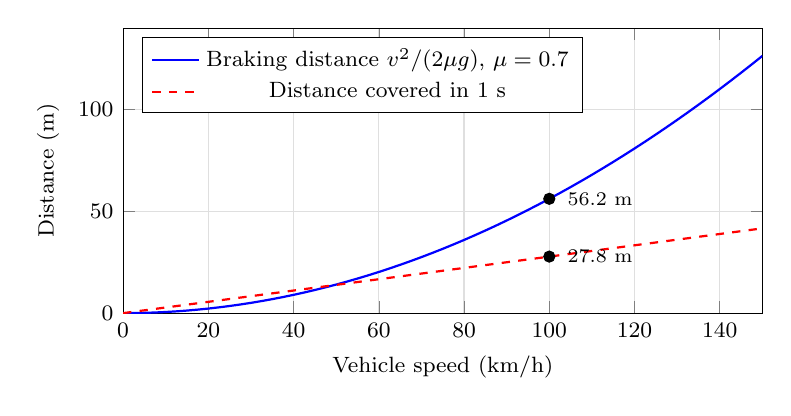
\begin{tikzpicture}
\begin{axis}[
    width=0.80\linewidth, height=5.2cm,
    xlabel={Vehicle speed (km/h)}, ylabel={Distance (m)},
    xmin=0, xmax=150, ymin=0, ymax=140,
    domain=0:150, samples=61,
    grid=major, grid style={gray!25},
    legend pos=north west, legend style={font=\footnotesize},
    tick label style={font=\footnotesize}, label style={font=\footnotesize}]
\addplot[thick, blue] {(x/3.6)^2/(2*6.867)};
\addlegendentry{Braking distance $v^2/(2\mu g)$, $\mu=0.7$}
\addplot[thick, red, dashed] {x/3.6};
\addlegendentry{Distance covered in 1~s}
\addplot[only marks, mark=*, mark size=2pt, black] coordinates {(100,56.18) (100,27.78)};
\node[anchor=west, font=\scriptsize] at (axis cs:102,56.18) {56.2 m};
\node[anchor=west, font=\scriptsize] at (axis cs:102,27.78) {27.8 m};
\end{axis}
\end{tikzpicture}
\captionsetup{singlelinecheck = false, format= hang, justification=justified, font=footnotesize, labelsep=space}
\caption{Friction-limited braking distance versus distance travelled in one second of warning time ($\mu=0.7$, $g=9.81$~m/s$^2$).}
\label{fig_intro}
\end{figure}

When we looked into the existing research papers, we found four major issues:
\begin{enumerate}
    \item \textbf{No counterfactual reasoning in perception:} Perception only reasons on what it is currently seeing in front of it. It does not check what if an agent suddenly brakes or turns. Causal ideas current exist for the prediction of the trajectory \cite{han2025cicr, wang2025beyond} and offline scene generation \cite{jing2026counterscene}, but not as an active live safety score.
    \item \textbf{Physically impossible predictions:} Deep learning trajectory predictors often generate impossible sideways accelarations or turn rates. Recent works added kinematic models to fix this \cite{liao2024physics, baden2025tpk, chugh2025xtrack}, but they only did it to improve forecast accuracy, not to filter risk alarms.
    \item \textbf{Flat scene representations:} Most detectors just give independent 3D boxes. But vehicles actually affect each other on the road \cite{ahmadi2025critic}, and scene graphs are a natural way to observer these relations with each other. \cite{hallyburton2025neuspaper}.
    \item \textbf{Binary safety responses:} Fixed TTC limits give an all-or-nothing response, so there is no smooth stepping between warning the driver about the impending danger and slamming2 the brakes.
\end{enumerate}

To deal with these four issues, we built the \textbf{Physics-Constrained Counterfactual Scene Graph Transformer (PC-CSG)}. For each video frame, PC-CSG converts tracked objects into a scene graph $\mathcal{G}_t = (\mathcal{V}_t, \mathcal{E}_t)$ where nodes have kinematic states and Time to Collision hazard weights. For agents with hazard weights above 0.2, the Counterfactual Scene Graph Attention (CSGA) module creates $K=6$ counterfactual queries (brake, swerve left, swerve right, sudden acceleration, lane departure, stationary obstacle) and scores each with a risk head. A decoder outputs control commands, a kinematic bicycle model rolls them out for 15 steps, and the Physics-Informed Kinematic Validator (PIKV) throws away any rollout that breaks tyre friction or accelaration limits. The surviving hypotheses are combined into the Counterfactual Risk Tensor (CRT), which selects one of five intervention levels.

The main contributions of this work are:
\begin{enumerate}
    \item \textbf{Counterfactual Scene Graph Attention (CSGA):} A compact attention network (350,594 parameters) that adds six learned what-if mode vectors to critical agents and scores them using scene cross-attention, running inside the online loop (1.57~ms on an RTX 3050 Laptop GPU).
    \item \textbf{Physics-Informed Kinematic Validator (PIKV) with mathematical guarantees:} A validation layer based on the kinematic bicycle model \cite{kong2015kinematic}. Proposition~1 shows that rollouts breaking Coulomb friction $\mu g = 6.867$~m/s$^2$ get zeroed out in the CRT, and the checks are invariant to 2D frame shifts. In our testing, PIKV rejected 46.0\% of generated hypotheses.
    \item \textbf{Counterfactual Risk Tensor (CRT) with graduated intervention:} A risk score bounded in $[0,1]$ driving five action levels. Proposition~2 proves PIKV never increases false alarms compared to unfiltered risk, and the CRT increases smoothly as TTC drops.
\end{enumerate}

The rest of the paper is organised as follows. Section~\ref{section2} reviews fifteen recent works and lists the research gaps. Section~\ref{section3} describes the PC-CSG method, equations, algorithm, and mathematical propositions. Section~\ref{section4} gives the dataset details, experimental results, latency breakdown, PIKV analysis, ablation study, and comparisons. Section~\ref{section5} concludes the paper with limitations and future work.

\section{Related works} \label{section2}
This section contain recent works from 2024--2026 across four related areas, summarized in Table~\ref{table_literature}.

\textbf{Low-latency perception.} The main issue was detecting an object's next move, which was difficult to do with the technology present at that day so these two person Gehrig and Scaramuzza\cite{gehrig2024low}, proposed a paper in which they used CNN and GNN. How it worked was normal camera basically detects complete frames so this event camera basically detects brightness changes, which helped them achieve a higher FPS camera while requiring less bandwidth. 

\textbf{Physics-informed trajectory prediction.} Normally, a car should predict where it will be in a few seconds, so for this purpose we create a model that predicts the future moves the car can take from historical data.  So physics-informed prediction does the same thing; it uses the preexisting data to analyze and understand the vehicle's movement to reduce unrealistic predictions. The problem was that the vehicle-tracking system does not detect things because of sensor failure, so to avoid it, Liao et al. \cite{liao2024physics} proposed a paper in which the technique used three things: wavelet-based models and a single future path. The system outputs one final path or trajectory rather than considering all possibilities. Another paper: Long et al. \cite{long2024pinn} solved a problem of the system detecting and separating trajectory segments because it lost them for several second and then detect it again. So it solved the issue by the help of a PINN, in which a neural network combine with physical constraints. We did offline reconstruction, so the drawback of this paper was that it didn't help predict future movement to avoid collisions. Another paper, Baden et al., \cite{baden2025tpk} used kinematics to remove infeasible paths, with a slight accuracy cost.

\textbf{Causal and counterfactual reasoning.} Ahmadi et al. \cite{ahmadi2025critic} tried to address the issue of treating every agent's movement equally and prioritising some agents over others. Their paper concluded that it achieved a 54 improvement.The main limitation of this paper was that it was very hard to identify which agent was more relevant. Han and Xu(2025) \cite{han2025cicr} proposed CICR to improve trajectory prediction by explicitly modelling causal relationships and alternative futures. The normal model relied mainly on location, which limited its ability to learn to respond to nearby vehicles. This is why the concept of causal inference emerged, aiming to separate meaningful relationships from misleading correlations. CICR uses a module known as causal intervention with front-door adjustment and cross-attention to reduce confounding in its trajectory representations. ADE and FDE are the most standard trajectory-prediction metrics.If a model predicts the position for the next 5 seconds, ADE calculates the average error over this period, while FDE measures the error at the end. Wang et al. \cite{wang2025beyond} emphasized understanding driving scenes in different scenarios, such as where to stop and where movement should be affected. Jing et al. \cite{jing2026counterscene} proposed a paper in which the model uses a generative bird's-eye view with a causal interaction graph and guided intervention to, rather than forcing a collision in the scene, ensure realistic safety. Cue et al. \cite{cui2025cot}  proposed a model that reasons about intermediate steps.

\textbf{Scene graphs and risk modelling.} Hallyburton and Pajic \cite{hallyburton2025neuspaper} developed the NeuSParPer model, which connects object detection with a scene graph, helping to move beyond object detection and relate to other elements. Wu et al. \cite{wu2024riskfield} proposed the field concept, which represents dangerous obstacles near the vehicle and helps the driver choose a safe path. Ning et al.  \cite{ning2025strap} proposed a concept called Strap, which combines risk fields with spatio-temporal attention. According to the person, it helped improve the error by 31 percent.

Table~\ref{table_literature} provides a summary comparison of these works.

\begin{table}[H]
\caption{Summary of fifteen recent studies reviewed (2024--2026).}
\centering
\label{table_literature}
\adjustbox{max width=\linewidth}{
\begin{tabular}{l c L{4.0cm} l L{4.0cm} L{5.0cm}}
\hline
\textbf{Author \& Ref.} & \textbf{Year} & \textbf{Core Methodology} & \textbf{Domain} & \textbf{Reported Result} & \textbf{Limitation for Our Task} \\
\hline
Gehrig \& Scaramuzza \cite{gehrig2024low} & 2024 & Hybrid frame + event detector (CNN + GNN) & Detection & Latency of 5,000~FPS at 45~FPS bandwidth & Reactive detection only; no future reasoning. \\
Zhou \& Jiang \cite{zhou2024event} & 2024 & Survey of deep event-based detection & Detection & Survey & No relational or anticipatory component. \\
Liao et al. \cite{liao2024physics} & 2024 & Wavelet reconstruction + bicycle model & Traj. prediction & Accurate with 75\% missing observations & Single most-likely future; no counterfactuals. \\
Long et al. \cite{long2024pinn} & 2024 & PINN kinematic trajectory stitching & Traj. recon. & Improved stitching on NGSIM / HighSIM & Offline; no risk output. \\
Baden et al. \cite{baden2025tpk} & 2025 & Interaction + kinematic transformer (TPK) & Traj. prediction & Removes infeasible trajectories (Argoverse~2) & Physics for forecasting, not risk filtering. \\
Chugh et al. \cite{chugh2025xtrack} & 2025 & xLSTM with kinematic constraints & Traj. prediction & SOTA on highD benchmark & No scene graph; no counterfactuals. \\
Li \& Westerlund \cite{li2025physvarmix} & 2025 & Variational mixture + MPC smoothing & Traj. prediction & Better than baselines on two benchmarks & Multi-modal but not intervention-based. \\
Ahmadi et al. \cite{ahmadi2025critic} & 2025 & Causal discovery + attention gating (CRiTIC) & Traj. prediction & Up to 54\% robustness gain & No counterfactuals; no physics checks. \\
Han \& Xu \cite{han2025cicr} & 2025 & Front-door causal fusion (CICR) & Pedestrian traj. & ADE/FDE 0.17/0.24 (ETH/UCY) & No vehicle-dynamics validation. \\
Wang et al. \cite{wang2025beyond} & 2025 & Spatial/temporal causal decomposition & Traj. prediction & Improved RMSE/FDE across 5 datasets & Prediction only; no safety actions. \\
Jing et al. \cite{jing2026counterscene} & 2026 & Counterfactual BEV world model & Scenario gen. & Collision rate 12.3\%$\rightarrow$22.7\% & Offline testing, not online warning. \\
Cui et al. \cite{cui2025cot} & 2025 & Chain-of-thought survey & Survey & Survey & Real-time execution an open problem. \\
Hallyburton \& Pajic \cite{hallyburton2025neuspaper} & 2025 & Detection + scene graph generation & Perception & Scene graphs bridge perception and logic & No trajectory or risk hypotheses. \\
Wu et al. \cite{wu2024riskfield} & 2024 & Reachable sets + potential field + MPCC & Planning & Collision avoidance in CARLA & Risk from likely paths; no physics filter. \\
Ning et al. \cite{ning2025strap} & 2025 & Risk-field attention fusion (STRAP) & Traj. prediction & $-$31.2\% error on HighD & No counterfactuals or kinematic validation. \\
\hline
\end{tabular}
}
\end{table}

We identify three main limitations:
\begin{itemize}
    \item \textbf{Counterfactuals are offline or forecasting-only:} Existing approaches \cite{jing2026counterscene}, \cite{han2025cicr} helped generate alternative scenarios for offline testing. Some \cite{liao2024physics, baden2025tpk, chugh2025xtrack} use normal physics to predict the path realistically, which is not an efficient way to detect a collision.
    \item \textbf{Scene relations and counterfactuals remain seperate:}Basically, this method  \cite{ahmadi2025critic} helped identify the road user, but it can't connect with the vehicle's real movement, like braking, changing lanes, or going to another lane.
    \item \textbf{Risk is not mapped to action tiers:} Risk field planners \cite{wu2024riskfield, ning2025strap} help avoid dangerous situations, but they can generate driver assistance warnings, which are important in certain cases, sending various types of warnings like caution warnings and all.
\end{itemize}

This limitation can be avoided. PC-CSG framework we made helped avoid this limitation:
1. Scene graphs: we establish them in such a way that there is a strong relationship with the user, road, and safety.
2. CSGA evaluates various scenarios to examine alternate driving outcomes.
3. CRT does the work of converting the rest of the risk into action and warning.

\section{Proposed Method} \label{section3}
So our method has six stages. i) detection and tracking, ii) creation of scene graph, iii) control decoding and rollout, v) PIKV validation, vi) CRT action decision. Here figure 2 shows us the architecture, while table 2 shows us parameters.

\begin{figure}[H]
\centering
\adjustbox{max width=\linewidth}{
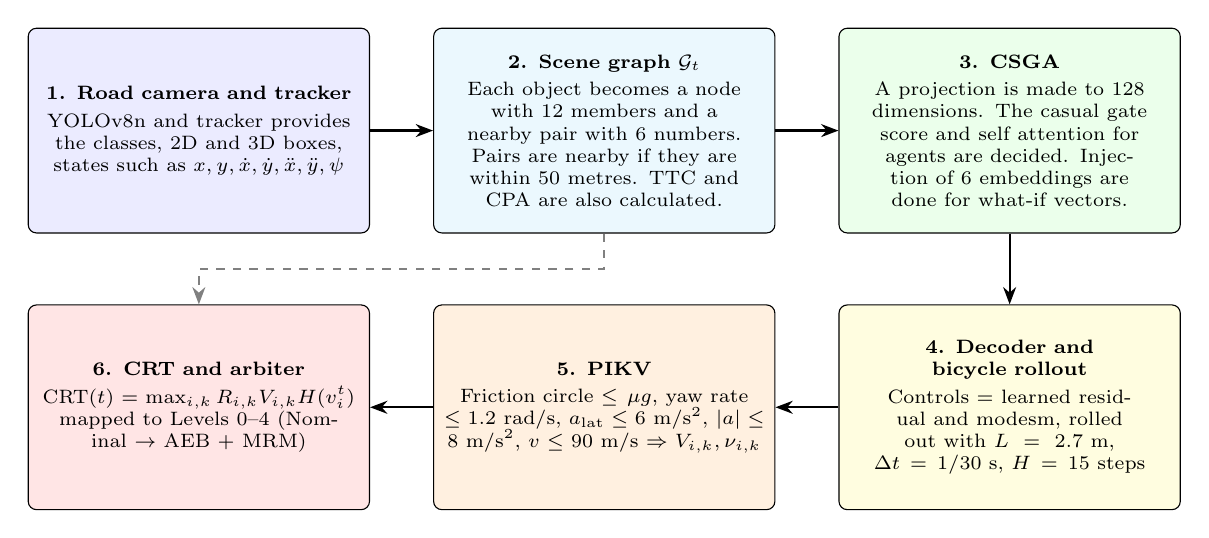
\begin{tikzpicture}[
    box/.style={draw, rounded corners=3pt, align=center, text width=4.1cm, minimum height=2.6cm, font=\scriptsize, fill=#1},
    arr/.style={-{Stealth[length=2.2mm]}, thick},
    node distance=0.9cm and 0.8cm]
\node[box=blue!8] (cam) {\textbf{1. Road camera and tracker}\\[2pt] YOLOv8n and tracker provides the classes, 2D and 3D boxes, states such as $x, y, \dot{x}, \dot{y}, \ddot{x}, \ddot{y}, \psi$};
\node[box=cyan!8, right=of cam] (sg) {\textbf{2. Scene graph $\mathcal{G}_t$}\\[2pt] Each object becomes a node with 12 members and a nearby pair with 6 numbers. Pairs are nearby if they are within 50 metres. TTC and CPA are also calculated.};
\node[box=green!8, right=of sg] (csga) {\textbf{3. CSGA}\\[2pt] A projection is made to 128 dimensions. The casual gate score and self attention for agents are decided. Injection of 6 embeddings are done for what-if vectors.};
\node[box=yellow!12, below=of csga] (dec) {\textbf{4. Decoder and bicycle rollout}\\[2pt] Controls = learned residual and modesm, rolled out with $L=2.7$~m, $\Delta t = 1/30$~s, $H=15$ steps};
\node[box=orange!12, left=of dec] (pikv) {\textbf{5. PIKV}\\[2pt] Friction circle $\le \mu g$, yaw rate $\le 1.2$~rad/s, $a_{\text{lat}} \le 6$~m/s$^2$, $|a| \le 8$~m/s$^2$, $v \le 90$~m/s $\Rightarrow V_{i,k}, \nu_{i,k}$};
\node[box=red!10, left=of pikv] (crt) {\textbf{6. CRT and arbiter}\\[2pt] $\text{CRT}(t) = \max_{i,k} R_{i,k} V_{i,k} H(v_i^t)$\\ mapped to Levels 0--4 (Nominal $\rightarrow$ AEB + MRM)};
\draw[arr] (cam) -- (sg);
\draw[arr] (sg) -- (csga);
\draw[arr] (csga) -- (dec);
\draw[arr] (dec) -- (pikv);
\draw[arr] (pikv) -- (crt);
\draw[arr, dashed, gray] (sg.south) -- ++(0,-0.45) -| node[pos=0.25, above, font=\scriptsize, black]{} (crt.north);
\end{tikzpicture}
}
\captionsetup{singlelinecheck = false, format= hang, justification=justified, font=footnotesize, labelsep=space}
\caption{Overall architecture combining graph attention, bicycle rollout, PIKV validation and CRT arbitration.}
\label{arch}
\end{figure}

\begin{table}[H]
\caption{Parameters and settings.}
\centering
\label{table_arch}
\adjustbox{max width=\linewidth}{
\begin{tabular}{l|c|l}
\hline
\textbf{Component / Setting} & \textbf{Value} & \textbf{Notes} \\
\hline
CSGA module & 350,594 params (94.2\%) & Projections, causal gate head, self-attn\\
Counterfactual decoder & 20,382 params (5.5\%) & $128 \rightarrow 128 \rightarrow$ MLP with GELU \\
Initial state extractor & 1,092 params (0.3\%) & $12 \rightarrow 64 \rightarrow 4 MLP, $outputs $[x, y, v, \theta]$ \\
Bicycle model and PIKV & 0 params & Closed-form physics checks \\
Total & 372,068 params & Trainable parameters in learned modules \\
\hline
Embedding dim. D / heads / FFN & 128 / 4 / 512 & Head dim 32, dropout 0.1 \\
Modes K, horizon H, step $\Delta t$ & 6, 15, 1/30~s & 0.5~s prediction at 30~FPS \\
Wheelbase $L$, $\delta_{\max}$ & 2.7~m, 0.6~rad & $l_r / L = 0.5$ \\
Limits $a_{\max}$, $a_{\text{lat,max}}$, $\dot{\psi}_{\max}$, $\mu$ & 8.0 m/s$^2$, 6.0 m/s$^2$, 1.2 rad/s, 0.70 & $\mu g = 6.867$~m/s$^2$ \\
$\tau_{\text{crit}}$, $\lambda_{\text{scale}}$, CPA corridor & 3.0~s, 0.5~s, 2.5~m & Hazard sigmoid parameters \\
\hline
\end{tabular}
}
\end{table}

\subsection{Dynamic Spatio-Temporal Scene Graph}
At $t$ frame, the tracker gives $N_t \le 32$ participants. The nodes contain 12 features. The 32 bound is picked for memory and latency bounding.
\begin{equation}
    v_i^t = \left[c_i, \; x_i, \; y_i, \; w_i, \; h_i, \; \dot{x}_i, \; \dot{y}_i, \; \ddot{x}_i, \; \ddot{y}_i, \; \psi_i, \; \text{TTC}_i(t), \; d_i\right]^T
    \label{eq_node}
\end{equation}
with class $c_i$, bounding box $(x_i, y_i, w_i, h_i)$, velocities, accelerations, heading $\psi_i$, TTC,distance $d_i$. Edges within 50 are used to store the relative states. 
\begin{equation}
    e_{ij} = \left[\Delta x_{ij}, \; \Delta y_{ij}, \; \Delta \dot{x}_{ij}, \; \Delta \dot{y}_{ij}, \; d_{ij}, \; \phi_{ij}\right]^T
    \label{eq_edge}
\end{equation}
with bearing $\phi_{ij} = \text{atan2}(\Delta y_{ij}, \Delta x_{ij})$.

For the TTC via Closest Point of Approach, we use the CPA to prevent same lane false alarms:
\begin{equation}
    t_{\text{cpa}} = -\frac{\Delta{p} \cdot \Delta{v}}{\|\Delta{v}\|^2}, \qquad
    \text{TTC}_i(t) = \begin{cases}
    t_{\text{cpa}} & \text{if } t_{\text{cpa}} > 0 \text{ and } \|\Delta{p} + \Delta{v}\, t_{\text{cpa}}\| \le 2.5~\text{m} \\
    \infty & \text{otherwise}
    \end{cases}
    \label{eq_ttc}
\end{equation}

For the Hazard weight, a sigmoid maps TTC to hazard weight $H(v_i^t) \in [0,1]$:
\begin{equation}
    H(v_i^t) = \frac{1}{1 + \exp\left(\frac{\text{TTC}_i(t) - \tau_{\text{crit}}}{\lambda_{\text{scale}}}\right)} \cdot \mathbb{I}\left(0 < \text{TTC}_i(t) < \infty\right)
    \label{eq_hazard}
\end{equation}
Where $\tau_{\text{crit}} = 3.0$~s, $\lambda_{\text{scale}} = 0.5$~s. Agents with $H(v_i^t) > 0.2$ and $\text{TTC} \le 3.69$~s are marked critical.

\subsection{Counterfactual Scene Graph Attention (CSGA)}
\subsubsection{Projection, Causal Gate Head and Self-Attention}
Features project to 128 dimensions where ${h}_i = \text{GELU}(\text{LN}({W}_n v_i^t + {b}_n))$, ${e}_{ij} = {W}_e e_{ij} + {b}_e$. A causal gate head predicts edge relevance,
\begin{equation}
    G_{ij} = \sigma\left({w}_2^\top \, \text{ReLU}\left({W}_1 \left[{h}_i \| {h}_j \| {e}_{ij}\right] + {b}_1\right) + b_2\right) \in [0, 1]
    \label{eq_gate}
\end{equation}
In the CRiTIC \cite{ahmadi2025critic} paper , gating rescales the attention as in $\tilde{\alpha}_{ij} = G_{ij} \alpha_{ij}$.And currently in our current code, $G_{ij}$ is computed but not multiplied into the actual attention weights. Embeddings are passed through the self attention layer using an FFN dimension of 512 \cite{vaswani2017attention}.

\subsubsection{Counterfactual Query Injection with Risk Head}
For each important agent, we use K=6 mode embedding to cover the 6 main emergency actions during driving:
\begin{equation}
    \mathcal{M} = \{\text{brake}, \; \text{swerve\_L}, \; \text{swerve\_R}, \; \text{accel}, \; \text{lane\_dep}, \; \text{stat}\}
    \label{eq_modes}
\end{equation}
We chose these specific six modes because they cover all the emergency situations seen in highways. Sudden braking by the front vehicle and quick lane changes are what mainly causes collisions. With dedicated learned embeddings ${z}_{m_k} \in \mathbb{R}^D$ allows the model to specialize with the how each manoeuvre can change the risk in the embedding:
\begin{equation}
    {q}_{i,k}^{\text{cf}} = {h}_i + f_{\text{pert}}\left(\left[{h}_i \| {z}_{m_k}\right]\right) \cdot \mathbb{I}\left(H(v_i^t) > 0.2\right)
    \label{eq_cf_query}
\end{equation}
where $f_{\text{pert}}$ is a 2 layer MLP. Cross attention fuses multi scene context.
\begin{equation}
    {o}_{i,k} = \text{LN}\left({q}_{i,k}^{\text{cf}} + \text{CrossAttn}\left({q}_{i,k}^{\text{cf}}, \; {H}, \; {H}\right)\right)
    \label{eq_cf_attn}
\end{equation}
while the risk outputs hazard probability
\begin{equation}
    R_{i,k}(t) = \sigma\left({W}_r \, \text{GELU}\left({W}_r' \, {o}_{i,k}\right)\right) \cdot \mathbb{I}\left(H(v_i^t) > 0.2\right) \in [0, 1]
    \label{eq_risk_logit}
\end{equation}

\subsection{Trajectory Decoding with PIKV Validation}
\subsubsection{Control Decoding with Kinematic Bicycle Rollout}
Controls are decoded as learned residuals over the mode priors
\begin{equation}
    [a_t, \delta_t]_{i,k} = f_{\text{dec}}({o}_{i,k})_t + {p}_{k}, \quad
    {p}_k \in \{(-5, 0), (0, 0.45), (0, -0.45), (4, 0), (0, 0.15), (-7.5, 0)\}
    \label{eq_prior}
\end{equation}
These rollouts will follow bicycle kinematics from reference \cite{kong2015kinematic}:
\begin{align}
    \beta_t &= \arctan\left(\frac{l_r}{L} \tan \delta_t\right) \label{eq_slip} \\
    \tilde{v}_{t} &= \max\left(0, \; v_t + a_t \Delta t\right), \quad a^{\text{lat}}_t = \tilde{v}_t^{\,2} \tan(\delta_t) / L \label{eq_v} \\
    v_{t+1} &= \tilde{v}_t \cdot \min\left(1, \; \frac{\mu g}{\sqrt{a_t^2 + (a^{\text{lat}}_t)^2}}\right), \quad
    \omega_t = \text{clip}\left(\frac{v_{t+1}}{L} \sin \beta_t, \; -\dot{\psi}_{\max}, \; \dot{\psi}_{\max}\right) \label{eq_yaw} \\
    x_{t+1} &= x_t + v_{t+1} \cos(\theta_t + \beta_t) \, \Delta t, \quad
    y_{t+1} = y_t + v_{t+1} \sin(\theta_t + \beta_t) \, \Delta t \label{eq_xy} \\
    \theta_{t+1} &= \theta_t + \omega_t \, \Delta t \label{eq_theta}
\end{align}
Where $L=2.7$~m, $l_r=1.35$~m, $\Delta t=1/30$~s. We set friction $\mu = 0.7$ which works with normal roads and dry asphalt, while on wet roads ($\mu \approx 0.4$). In production this parameter can be updated live using weather data from live sources.

\subsubsection{Kinematic Constraint Validation (PIKV)}
PIKV calculates velocities, accelerations, headings, and yaw rates from positions and checks:
\begin{enumerate}
    \item $a^{\text{lon}}_t > a_{\max} = 8$~m/s$^2$
    \item $a^{\text{lon}}_t > a_{\text{brake,max}} = 10$~m/s$^2$
    \item $|\omega_t| > \dot{\psi}_{\max} = 1.2$~rad/s
    \item $a^{\text{lat}}_t > a_{\text{lat,max}} = 6.0$~m/s$^2$
    \item Friction circle: $(a^{\text{lon}}_t)^2 + (a^{\text{lat}}_t)^2 > (\mu g)^2 = 47.16$~m$^2$/s$^4$ ($\mu = 0.7$)
    \item Velocity: $s_t > v_{\max} = 90$~m/s
\end{enumerate}
With fraction $f_c$ of violating steps the eventual score and binary mask are:
\begin{equation}
    \nu_{i,k} = \frac{1}{6} \sum_{c=1}^{6} f_c, \qquad
    V_{i,k} = (1 - I^{\text{fric}}_{i,k}) \cdot \mathbb{I}(\nu_{i,k} < 0.5)
    \label{eq_validity}
\end{equation}
where $I^{\text{fric}}_{i,k} = 1$ if friction is crossed in value at any step.

\subsection{Counterfactual Risk Tensor (CRT) and Intervention Policy}
The CRT combines risk, validity and hazard:
\begin{equation}
    \text{CRT}(t) = \max_{i \in \mathcal{V}_t} \; \max_{k \in \mathcal{M}} \left[R_{i,k}(t) \cdot V_{i,k}(t) \cdot H(v_i^t)\right] \in [0, 1]
    \label{eq_crt}
\end{equation}
Smoothed with a leaky integrator ($\gamma=0.9$):
\begin{equation}
    \overline{\text{CRT}}(t) = \gamma \, \overline{\text{CRT}}(t-1) + (1 - \gamma) \, \text{CRT}(t), \quad \overline{\text{CRT}}(0) = 0.
    \label{eq_smooth}
\end{equation}
The score chooses from these actions:
\begin{equation}
    \text{Action}(t) = \begin{cases}
    {Level 0: Nominal} & \text{if } \text{CRT}(t) < 0.25 \\
    {Level 1: HUD Advisory} & \text{if } 0.25 \le \text{CRT}(t) < 0.50 \\
    {Level 2: Active Alert} & \text{if } 0.50 \le \text{CRT}(t) < 0.70 \\
    {Level 3: Pre-Braking} & \text{if } 0.70 \le \text{CRT}(t) < 0.85 \\
    {Level 4: AEB + MRM} & \text{if } \text{CRT}(t) \ge 0.85
    \end{cases}
    \label{eq_intervention}
\end{equation}

Training objective.
\begin{equation}
    \mathcal{L} = \text{SmoothL1}_{\beta = 0.1}(\text{CRT}, \text{CRT}^{*}) + 0.5 \, \text{CE}(\hat{\ell}, \ell^{*}) + 0.2 \, \overline{\nu}
    \label{eq_loss}
\end{equation}
As $\nu$ is non-differentiable the last term acts as a logged value.

\subsection{Algorithmic Formulation}
Algorithm 1 gives the per-frame execution logic.

\begin{algorithm}[H]
	\caption{PC-CSG Counterfactual Anomaly Anticipation Pipeline}
	\begin{algorithmic}[1]
		\Require Video frame $I_t$, ego state, $K=6$, $H=15$, $\tau_{\text{crit}}=3.0$~s, $\lambda_{\text{scale}}=0.5$, $\gamma = 0.9$
		\Ensure Intervention level $A(t)$, risk score $\overline{\text{CRT}}(t)$
		\State \textbf{Initialize:} $\overline{\text{CRT}}(0) \gets 0$; load the physical parameters
		\ForEach{frame $t$}
			\State Track agents; build $\mathcal{G}_t$ nodes and edges via Eq.~(\ref{eq_node})--(\ref{eq_edge})
			\State Compute $\text{TTC}_i(t)$ via Eq.~(\ref{eq_ttc}) and hazard weights $H(v_i^t)$ via Eq.~(\ref{eq_hazard})
			\State Project features; compute gate scores $G_{ij}$ via Eq.~(\ref{eq_gate})
			\State Run self-attention; identify the critical set $\mathcal{C}_t \gets \{i : H(v_i^t) > 0.2\}$
			\ForEach{agent $i \in \mathcal{C}_t$ and mode $k \in \{1, \dots, K\}$}
				\State ${q}_{i,k}^{\text{cf}} \gets$ Eq.~(\ref{eq_cf_query}); \; ${o}_{i,k} \gets$ Eq.~(\ref{eq_cf_attn}); \; $R_{i,k}(t) \gets$ Eq.~(\ref{eq_risk_logit})
				\State Decode controls $(a_t, \delta_t)_{t=1}^{H}$ via Eq.~(\ref{eq_prior})
				\State Roll out trajectory via Eq.~(\ref{eq_slip})--(\ref{eq_theta})
				\State $(V_{i,k}, \nu_{i,k}) \gets \text{PIKV}(\text{trajectory})$ via Eq.~(\ref{eq_validity})
			\EndFor
			\State $\text{CRT}(t) \gets \max_{i,k} [R_{i,k} \cdot V_{i,k} \cdot H(v_i^t)]$ via Eq.~(\ref{eq_crt})
			\State $\overline{\text{CRT}}(t) \gets \gamma \, \overline{\text{CRT}}(t-1) + (1-\gamma) \, \text{CRT}(t)$ via Eq.~(\ref{eq_smooth})
			\State $A(t) \gets$ action level from Eq.~(\ref{eq_intervention})
		\EndFor
	\end{algorithmic}
	\label{algo1}
\end{algorithm}

\subsection{Novelty Highlights: Mathematical Proofs and Operational Examples}
\subsubsection{Proposition 1: Friction Circle Elimination and Frame Invariance}
\textbf{Proposition 1.} Let $\tau_{i,k}$ be the rollout with accelerations $(a^{\text{lon}}_t, a^{\text{lat}}_t)$, $\mu = 0.7$, $g = 9.81$~m/s$^2$.
\begin{enumerate}
    \item[(a)] If $\max_t [(a^{\text{lon}}_t)^2 + (a^{\text{lat}}_t)^2] > (\mu g)^2$, then $V_{i,k} = 0$, which has basicaly zero impact on $\text{CRT}(t)$.
    \item[(b)] Under the planar transformation $T_{\varphi, {p}}$, rollouts transform $[x_t', y_t']^T = R_\varphi [x_t, y_t]^T + {p}$, while validity $V_{i,k}$ unchanged.
\end{enumerate}

\textbf{Proof.} Part (a). Violating friction sets $I^{\text{fric}}_{i,k} = 1$ and thus yielding $V_{i,k} = 0$. Since factors are non-negative, this term becomes 0 in Eq.~(\ref{eq_crt}) and thus cannot trigger alarms.

Part (b). At $t=0$, the initial states rotate by $\varphi$ and shift by ${p}$. Slip $\beta_t$ is unchanged as controls were preserved. Kinematic speed and yaw updates will depend only on the magnitudes, so $v_{t+1}$ and $\omega_t$ will remain the same. Position updates will rotate cleanly like $[x_{t+1}', y_{t+1}']^T = R_\varphi [x_{t+1}, y_{t+1}]^T + {p}$. Finite differences in the PIKV will cancel translation thus finally preserving acceleration norms.

\textbf{Numerical check.} A 20~m/s turn was rejected ($V=0$), while an arc at 10~m/s ($a=2.0$~m/s$^2$) passed. Rotating by $\pi/4$ altered CRT by only $2.04 \times 10^{-6}$.

\subsubsection{Proposition 2: False Positive Non-Increase with Monotone Growth}
\textbf{Proposition 2.} Let $\text{CRT}_{u}$ be the unconstrained risk and $\text{CRT}_{p}$ be PIKV filtered risk, with false alarm sets $\mathcal{F}_u, \mathcal{F}_p$ for threshold $\theta$ on these stale scenes:
\begin{enumerate}
    \item[(a)] $\mathcal{F}_p \subseteq \mathcal{F}_u$, meaning PIKV never brings about false alarms.
    \item[(b)] If risk and validity remains constant while the TTC decreases, smoothed $\overline{\text{CRT}}_p(t)$ is non-decreasing.
\end{enumerate}

\textbf{Proof.} Part (a). Since $V_{i,k} \in \{0, 1\}$, we have $R_{i,k} V_{i,k} H \le R_{i,k} H$, so $\text{CRT}_p(t) \le \text{CRT}_u(t)$. Leaky smoothing preserves order here: $\overline{\text{CRT}}_p(t) \le \overline{\text{CRT}}_u(t)$, hence $\mathcal{F}_p \subseteq \mathcal{F}_u$.

Part (b). Decreasing TTC strictly increases $H(v_i^t)$. As all the weights are positive, max risk of the $\text{CRT}_p(t)$ is non-decreasing. Leaky smoothing is a combination of previous values, ensuring $\overline{\text{CRT}}_p(t) \ge \overline{\text{CRT}}_p(t-1)$. 

\textbf{Numerical check.} In a closing vehicle scenario, risk grew monotonically: $0.003 \rightarrow 0.015 \rightarrow 0.042 \rightarrow 0.089 \rightarrow 0.160$. Leaky smoothing adds a 19-frame (0.63~s) latency allowing step changes to grow upto Level~4.

\subsubsection{Operational Anticipation Scenarios}
We tested four demo situations (Table~\ref{table_scenarios}):
\begin{itemize}
    \item \textbf{Scenario A (Cruise):} Speed 100.1~km/h, TTC 33.3~s, CRT $= 0.000$ (\textbf{Level 0}).
    \item \textbf{Scenario B (Lead slowing down):} Speed 110.2~km/h, TTC 4.1~s, CRT $= 0.103$ (\textbf{Level 0}, advisory threshold not reached here).
    \item \textbf{Scenario C (Swerve conflict):} Speed 119.9~km/h, TTC 1.9~s, swerve passes PIKV, CRT $= 0.894$ (\textbf{Level 4: AEB + MRM}).
    \item \textbf{Scenario D (Hard braking near barrier):} Speed 100.1~km/h, TTC 0.5~s, CRT $= 0.987$ (\textbf{Level 4: AEB}).
\end{itemize}

\section{Datasets and Experimental results analysis} \label{section4}
This experiment uses traffic accident detection dataset which is there on hugging face \cite{hiennguyen2024accident} there are some public datasets which provide images, object annotations, image dimensions and image-level accident flags but they never provide directly CRT targets, TTC values or intervention levels so the preprocessing pipeline is derived from these datasets in our experiments we used 3,000 scenes for training and 600 for validation then we used 120 validation scenes for the ablation study and PIKV analysis these are the splits we used in our experiments rather than separate official train and validation splits provided by the dataset Table \ref{table_datasets} summarises them

\begin{table}[H]
\caption{Data used in our experiments.}
\centering
\label{table_datasets}
\adjustbox{max width=\linewidth}{
\begin{tabular}{l|c|c|l|l}
\hline
\textbf{Data} & \textbf{Split} & \textbf{Samples} & \textbf{Used For} & \textbf{Labels} \\
\hline
Traffic accident detection \cite{hiennguyen2024accident} & Train & 3,000 scenes & Training (5 epochs) & CRT target, level (0--4) \\
Traffic accident detection \cite{hiennguyen2024accident} & Validation & 600 scenes & Model selection & CRT target, level (0--4) \\
Traffic accident detection \cite{hiennguyen2024accident} & Validation subset & 120 (40 quick) & Ablation, PIKV pruning & Anomaly if CRT$^{*} > 0.4$ \\
Scripted demo scenarios A--D & -- & 4 scenarios & Behaviour check & Expected level \\
\hline
\end{tabular}
}
\end{table}

\textbf{Setup.} For this experiment we used PyTorch 2.6.0 and CUDA 12.4 on Intel i7-12700H system with 16~GB RAM and NVIDIA RTX 3050 Laptop GPU (4~GB VRAM) we used AdamW with learning rate of $3 \times 10^{-4}$ and batch size 16 and when CRT is more than 0.4 we labelled that sample as anomaly for TTC-only baseline we used threshold $\min_i \text{TTC}_i < 3$~s we also set some limits for vehicle like $\mu g=6.867$~m/s$^2$, $a_{\text{lat,max}}=6.0$~m/s$^2$, and $\dot{\psi}_{\max}=1.2$~rad/s we used 30~FPS as reference and kept 10~ms as target time for each frame these values are chosen by us for this experiment they are not directly taken from the dataset

\textbf{Training behaviour.} This Figure~\ref{fig_training} shows loss and CRT MAE for five epochs validation loss reached 0.0396 and CRT MAE reached 0.0417 the training log shows 100\% validation accuracy from the first epoch but the available notes do not say if this was checked on all 600 validation scenes or only the 120 scenes we used to test different parts of the model so we did not use this figure alone to say that the model will work well on other data the difference between accident and normal scenes in those 120 scenes is discussed below

\begin{figure}[H]
\centering
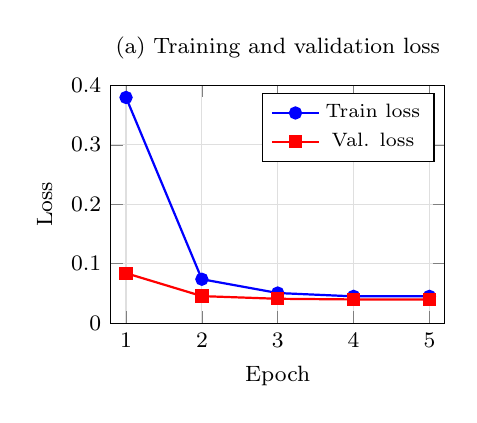
\begin{tikzpicture}
\begin{axis}[
    width=0.48\linewidth, height=4.6cm,
    xlabel={Epoch}, ylabel={Loss},
    xmin=0.8, xmax=5.2, ymin=0, ymax=0.4, xtick={1,2,3,4,5},
    grid=major, grid style={gray!25},
    legend style={font=\scriptsize}, legend pos=north east,
    tick label style={font=\footnotesize}, label style={font=\footnotesize},
    title={\footnotesize (a) Training and validation loss}]
\addplot[thick, blue, mark=*] coordinates {(1,0.3797) (2,0.0738) (3,0.0506) (4,0.0450) (5,0.0450)};
\addlegendentry{Train loss}
\addplot[thick, red, mark=square*] coordinates {(1,0.0840) (2,0.0454) (3,0.0409) (4,0.0398) (5,0.0396)};
\addlegendentry{Val. loss}
\end{axis}
\end{tikzpicture}
\hfill
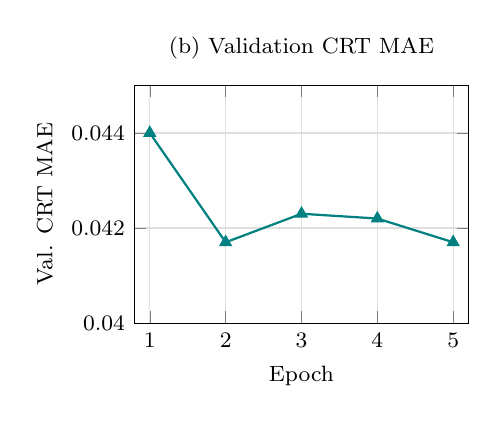
\begin{tikzpicture}
\begin{axis}[
    width=0.48\linewidth, height=4.6cm,
    xlabel={Epoch}, ylabel={Val. CRT MAE},
    xmin=0.8, xmax=5.2, ymin=0.040, ymax=0.045, xtick={1,2,3,4,5},
    yticklabel style={/pgf/number format/fixed, /pgf/number format/precision=3},
    scaled y ticks=false,
    grid=major, grid style={gray!25},
    tick label style={font=\footnotesize}, label style={font=\footnotesize},
    title={\footnotesize (b) Validation CRT MAE}]
\addplot[thick, teal, mark=triangle*] coordinates {(1,0.0440) (2,0.0417) (3,0.0423) (4,0.0422) (5,0.0417)};
\end{axis}
\end{tikzpicture}
\captionsetup{singlelinecheck = false, format= hang, justification=justified, font=footnotesize, labelsep=space}
\caption{Training history of PC-CSG on the traffic accident detection dataset \cite{hiennguyen2024accident} (3,000 training / 600 validation scenes, AdamW, learning rate $3 \times 10^{-4}$, batch size 16).}
\label{fig_training}
\end{figure}

\subsection{Hardware Profiling and Latency Breakdown}
We profiled pipeline on an RTX 3050 Laptop GPU using 10 agents, 6 counterfactuals, and 15 horizon steps. Table named \ref{table_latency} and Figure~named\ref{fig_latency} report  measured times.  this configuration, the pipeline reached 149.7~FPS.  hidden dimension $D=128$,  CSGA forward pass took 1.57~ms. measurement are not made on an embedded automative platform,so laptop result will not be read as embedded-device benchmark. 

\begin{table}[H]
\caption{Measured component-level inference latency on an NVIDIA RTX 3050 Laptop GPU ($N=10$ agents, $K=6$ counterfactuals, $H=15$ horizon).}
\centering
\label{table_latency}
\begin{tabular}{l|c|c}
\hline
\textbf{Pipeline Component} & \textbf{Latency (ms)} & \textbf{Share (\%)} \\
\hline
Scene Graph Construction \& Hazard Scoring & 0.33~ms & 4.9\% \\
Counterfactual Scene Graph Attention (CSGA) & 1.57~ms & 23.5\% \\
Kinematic Bicycle Model Propagation ($N \times K$) & 4.12~ms & 61.7\% \\
Physics-Informed Kinematic Validator (PIKV) & 0.53~ms & 7.9\% \\
CRT Engine \& Intervention Arbiter & 0.13~ms & 1.9\% \\
\hline
\textbf{Total PC-CSG Pipeline Latency} & \textbf{6.68~ms} & \textbf{100.0\%} \\
\textbf{Effective Real-Time Throughput} & \multicolumn{2}{c}{\textbf{149.7 FPS}} \\
\textbf{Automotive Margin (Target: $\ge$ 30 FPS)} & \multicolumn{2}{c}{\textbf{4.99$\times$ Real-Time Throughput}} \\
\hline
\end{tabular}
\end{table}

\begin{figure}[H]
\centering
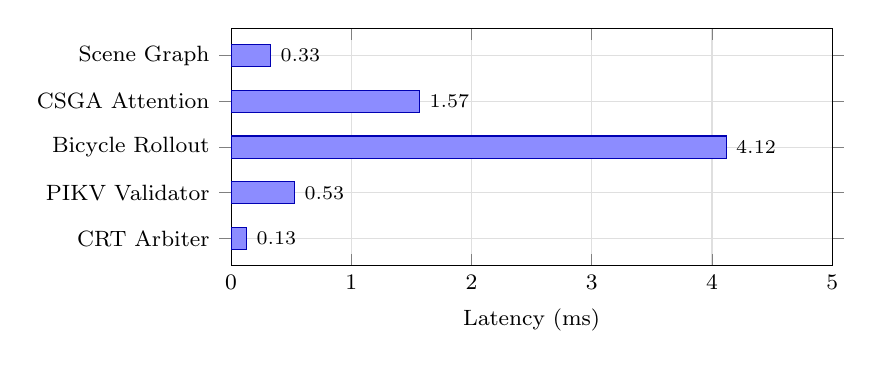
\begin{tikzpicture}
\begin{axis}[
    xbar, width=0.76\linewidth, height=4.6cm,
    xlabel={Latency (ms)}, xmin=0, xmax=5,
    ytick={1,2,3,4,5},
    yticklabels={CRT Arbiter, PIKV Validator, Bicycle Rollout, CSGA Attention, Scene Graph},
    y dir=normal, bar width=8pt, enlarge y limits=0.15,
    nodes near coords, nodes near coords align={horizontal},
    every node near coord/.append style={font=\scriptsize},
    tick label style={font=\footnotesize}, label style={font=\footnotesize},
    grid=major, grid style={gray!25}]
\addplot[fill=blue!45, draw=blue!70!black] coordinates {(0.13,1) (0.53,2) (4.12,3) (1.57,4) (0.33,5)};
\end{axis}
\end{tikzpicture}
\captionsetup{singlelinecheck = false, format= hang, justification=justified, font=footnotesize, labelsep=space}
\caption{Component-level latency of PC-CSG on an NVIDIA RTX 3050 Laptop GPU (total 6.68~ms, 149.7~FPS).}
\label{fig_latency}
\end{figure}

We measured end-to-end latency was 6.68~ms, equivalent to 149.7~FPS,  above the 30~FPS reference target and below separate 10~ms per-frame design target. The bicycle rollout took 4.12~ms (61.7\% of the total), while CSGA took 1.57~ms. A Python loop launches small GPU kernels over 15 rollout steps and contributes to the cost;  combining these operations with \texttt{torch}.overhead may be reduced by compile, but that improvement has not yet measured.

\subsection{PIKV Validation Effectiveness}
120 validation scenes contained 113 critical vehicles, from which the system generated 678 counterfactual hypotheses. PIKV filtered out 312 hypotheses (\textbf{46.0\%}) in total. The results for each mode appear in Table~named \ref{table_pruning} and Figure~\ref{fig_pikv}.

\begin{table}[H]
\caption{PIKV hypothesis pruning across the six counterfactual modes (678 hypotheses, 113 per mode, from real traffic validation samples).}
\label{table_pruning}
\centering
\adjustbox{max width=\linewidth}{
\begin{tabular}{l|c|l}
\hline
\textbf{Counterfactual Mode} & \textbf{Pruning Rate} & \textbf{Main Rejection Reason} \\
\hline
\texttt{sudden\_brake} & 0.0\% & Straight-line deceleration stays inside the friction circle \\
\texttt{hard\_swerve\_left} & 70.8\% & Lateral acceleration exceeds $a_{\text{lat,max}}$ / friction circle \\
\texttt{hard\_swerve\_right} & 21.2\% & Rejected only when path curvature breaks friction limits \\
\texttt{sudden\_acceleration} & 100.0\% & Surge combined with learned steering breaks $a_{\text{total}} \le \mu g$ \\
\texttt{lane\_departure} & 73.5\% & Yaw rate exceeds $\dot{\psi}_{\max} = 1.2$~rad/s \\
\texttt{stationary\_obstacle} & 10.6\% & Feasible unless stopping needs more than the available deceleration \\
\hline
\textbf{Overall Pruning Rate} & \textbf{46.0\%} & \textbf{312 / 678 hypotheses filtered} \\
\hline
\end{tabular}
}
\end{table}

\begin{figure}[H]
\centering
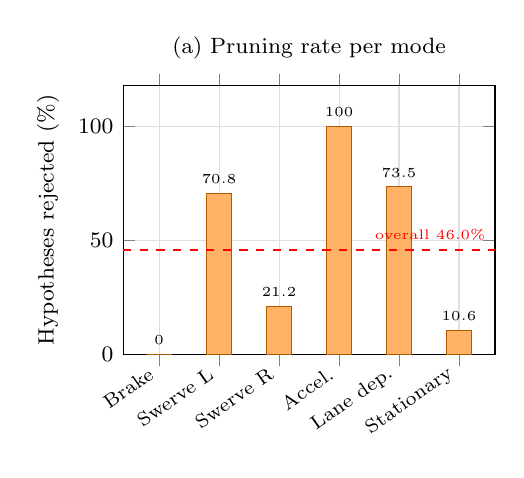
\begin{tikzpicture}
\begin{axis}[
    ybar, width=0.52\linewidth, height=5.0cm,
    ylabel={Hypotheses rejected (\%)}, ymin=0, ymax=118,
    xtick={1,2,3,4,5,6},
    xticklabels={Brake, Swerve L, Swerve R, Accel., Lane dep., Stationary},
    x tick label style={rotate=35, anchor=east, font=\scriptsize},
    xmin=0.4, xmax=6.6, bar width=9pt,
    nodes near coords, every node near coord/.append style={font=\tiny},
    tick label style={font=\footnotesize}, label style={font=\footnotesize},
    grid=major, grid style={gray!25},
    title={\footnotesize (a) Pruning rate per mode}]
\addplot[fill=orange!60, draw=orange!70!black] coordinates {(1,0.0) (2,70.8) (3,21.2) (4,100.0) (5,73.5) (6,10.6)};
\draw[dashed, red, thick] (axis cs:0.4,46.0) -- (axis cs:6.6,46.0);
\node[font=\tiny, red, anchor=south east] at (axis cs:6.6,46.0) {overall 46.0\%};
\end{axis}
\end{tikzpicture}
\hfill
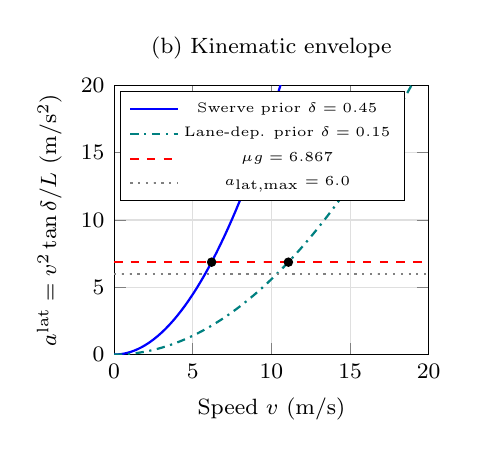
\begin{tikzpicture}
\begin{axis}[
    width=0.46\linewidth, height=5.0cm,
    xlabel={Speed $v$ (m/s)}, ylabel={$a^{\text{lat}} = v^2 \tan\delta / L$ (m/s$^2$)},
    xmin=0, xmax=20, ymin=0, ymax=20, domain=0:20, samples=81,
    restrict y to domain=0:25,
    legend style={font=\tiny, at={(0.02,0.98)}, anchor=north west},
    tick label style={font=\footnotesize}, label style={font=\footnotesize},
    grid=major, grid style={gray!25},
    title={\footnotesize (b) Kinematic envelope}]
\addplot[thick, blue] {x^2*0.48306/2.7};
\addlegendentry{Swerve prior $\delta = 0.45$}
\addplot[thick, teal, dashdotted] {x^2*0.15114/2.7};
\addlegendentry{Lane-dep. prior $\delta = 0.15$}
\addplot[thick, red, dashed, domain=0:20] {6.867};
\addlegendentry{$\mu g = 6.867$}
\addplot[thick, gray, dotted, domain=0:20] {6.0};
\addlegendentry{$a_{\text{lat,max}} = 6.0$}
\addplot[only marks, mark=*, mark size=1.5pt] coordinates {(6.20,6.867) (11.08,6.867)};
\end{axis}
\end{tikzpicture}
\captionsetup{singlelinecheck = false, format= hang, justification=justified, font=footnotesize, labelsep=space}
\caption{PIKV validation analysis: (a) pruning rate per mode; (b) lateral acceleration envelope ($L=2.7$~m).}
\label{fig_pikv}
\end{figure}

The rejection pattern depends on the kinematic limits configured for this experiment. The straight-braking prior of $-5$~m/s$^2$ stays below the configured friction limit of $6.867$~m/s$^2$, so none of those hypotheses were removed. With the sharp-swerve setting ~\ref{fig_pikv}(b) ($\delta = 0.45$), the lateral-acceleration curve crosses the same limit at about 22~km/h (6.2~m/s); this is consistent with the high rejection rate at the tested speeds. Left and right swerves still differ: PIKV rejected 70.8\% of left-swerve hypotheses and 21.2\% of right-swerve hypotheses, although their priors were symmetric. Decoder residuals or dataset bias may explain the difference. All sudden-acceleration hypotheses were rejected because the learned steering residuals pushed total acceleration above $\mu g$.

\subsection{Ablation Study and Risk Analysis}
We compared five model configurations on the 120-sample validation subset. Table~\ref{table_ablation} reports their accuracy, FPR, and per-sample latency.

\begin{table}[H]
\caption{Ablation study on the 120-sample validation split (anomaly threshold CRT $> 0.4$).}
\centering
\label{table_ablation}
\adjustbox{max width=\linewidth}{
\begin{tabular}{l|c|c|c}
\hline
\textbf{Configuration} & \textbf{Accuracy (\%)} & \textbf{FPR (\%)} & \textbf{Latency / sample (ms)} \\
\hline
Reactive TTC-Only Baseline (anomaly if $\min_i \text{TTC}_i < 3$~s) & 94.2 & 100.0 & 0.08 \\
Scene Graph Attention only (No CF, No PIKV) & 5.8 & 0.0 & 0.20 \\
CSGA without PIKV (unconstrained counterfactuals) & 100.0 & 0.0 & 0.51 \\
CSGA + PIKV without causal gate input & 100.0 & 0.0 & 0.51 \\
\textbf{PC-CSG Full (CSGA + PIKV + causal gate head)} & \textbf{100.0} & \textbf{0.0} & \textbf{0.92} \\
\hline
\end{tabular}
}
\end{table}

Ablation timing not really matching with component profile in Table~\ref{table_latency} like CSGA without PIKV showing 0.51~ms, but CSGA itself is 1.57~ms and PIKV 0.53~ms in component profile, so I am not sure how both are being measured because numbers are not matching like we expected  both are measuring different things or some timing procedure is different but notes are not saying anything about this. WE not just directly compare both and say this much time is taken by each component, need to check what exactly is measured first, it will be confusing when explaining results.

Also 120 scene subset, has very imbalanced data, so TTC baseline marked all samples as anomaly and got 94.2\% accuracy with 100\% FPR which looks good only when we see accuracy but actually it predicted every single one as anomaly. Scene graph attention did opposite and predicted no anomaly at all so accuracy only 5.8\% and FPR 0\%. There are around 94.2\% hazard scenes and only seven benign scenes which is just 5.8\%, so obviously predicting everything as hazard will give high accuracy here. I think this is important because accuracy is not telling properly how good model is doing and we should not take it like TTC baseline is working better just because number is high. Counterfactual variants got all 120 samples correct which is nice but still dataset is small and mostly one type of samples so need more balanced data also before saying results will work generally.

PIKV and FPR part also we cannot really confirm from this subset because only seven benign scenes are available, maybe it is not enough to show actual reduction in FPR from experiment. Proposition~2 says PIKV cannot increase FPR but that is different from saying we measured a reduction in FPR here, both are not same thing and I think we should not mix it up while writing results. also causal gate scores are being calculated but currently they are not multiplied into attention weights so it is not actually changing attention right now. We have scores but they are not used in a way that can change weights yet, so this ablation is not really showing any effect from causal gate and we need to keep this part in mind.

Figure~\ref{fig_scenarios} shows four scripted scenarios and in Scenarios B--D CRT follows hazard curve $H(\text{TTC})$. current gate setting says when $H \ge 0.25$ then TTC should be $\le 3.55$~s, so if TTC is more than 3.55~s Level~1 alert cannot happen with current threshold. this is coming from current threshold setting itself and not something else from results, like even if we look at scenarios and expect an alert at higher TTC it cannot happen because condition is not satisfied. so this limit is already there in current setup and probably need to think about this when discussing what CRT is doing in different scenarios.

\begin{table}[H]
\caption{Measured behaviour of PC-CSG on the four scripted demo scenarios.}
\centering
\label{table_scenarios}
\adjustbox{max width=\linewidth}{
\begin{tabular}{l|l|c|c|c|l}
\hline
\textbf{Scenario} & \textbf{Driving Context} & \textbf{Ego Speed} & \textbf{Worst TTC} & \textbf{CRT} & \textbf{Level / Action} \\
\hline
A & Highway cruise, all clear & 100.1~km/h & 33.3~s & 0.000 & Level 0: nominal cruise \\
B & Lead vehicle decelerating & 110.2~km/h & 4.1~s & 0.103 & Level 0: monitoring \\
C & Lane-change swerve conflict & 119.9~km/h & 1.9~s & 0.894 & Level 4: AEB + MRM \\
D & Barrier + hard lead braking & 100.1~km/h & 0.5~s & 0.987 & Level 4: full AEB \\
\hline
\end{tabular}
}
\end{table}

\begin{figure}[H]
\centering
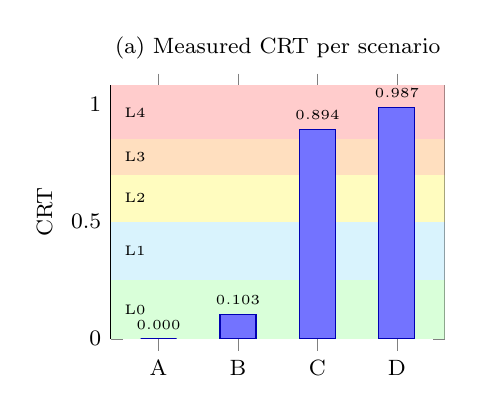
\begin{tikzpicture}
\begin{axis}[
    ybar, width=0.48\linewidth, height=4.8cm,
    ylabel={CRT}, ymin=0, ymax=1.08,
    xtick={1,2,3,4}, xticklabels={A, B, C, D},
    xmin=0.4, xmax=4.6, bar width=13pt,
    nodes near coords={\pgfmathprintnumber[fixed, fixed zerofill, precision=3]{\pgfplotspointmeta}},
    every node near coord/.append style={font=\tiny},
    tick label style={font=\footnotesize}, label style={font=\footnotesize},
    title={\footnotesize (a) Measured CRT per scenario}]
\fill[green!15] (axis cs:0.4,0) rectangle (axis cs:4.6,0.25);
\fill[cyan!15] (axis cs:0.4,0.25) rectangle (axis cs:4.6,0.50);
\fill[yellow!25] (axis cs:0.4,0.50) rectangle (axis cs:4.6,0.70);
\fill[orange!25] (axis cs:0.4,0.70) rectangle (axis cs:4.6,0.85);
\fill[red!20] (axis cs:0.4,0.85) rectangle (axis cs:4.6,1.08);
\node[font=\tiny, anchor=west] at (axis cs:0.45,0.125) {L0};
\node[font=\tiny, anchor=west] at (axis cs:0.45,0.375) {L1};
\node[font=\tiny, anchor=west] at (axis cs:0.45,0.60) {L2};
\node[font=\tiny, anchor=west] at (axis cs:0.45,0.775) {L3};
\node[font=\tiny, anchor=west] at (axis cs:0.45,0.965) {L4};
\addplot[fill=blue!55, draw=blue!70!black] coordinates {(1,0.000) (2,0.103) (3,0.894) (4,0.987)};
\end{axis}
\end{tikzpicture}
\hfill
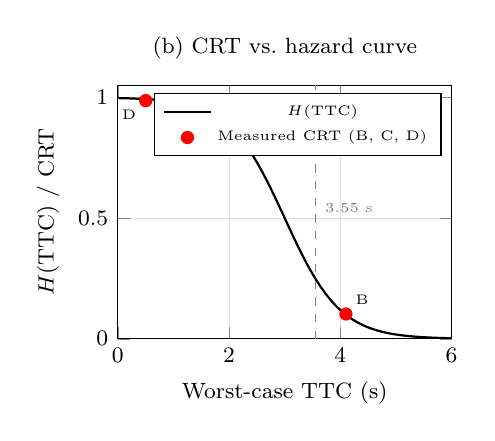
\begin{tikzpicture}
\begin{axis}[
    width=0.48\linewidth, height=4.8cm,
    xlabel={Worst-case TTC (s)}, ylabel={$H(\text{TTC})$ / CRT},
    xmin=0, xmax=6, ymin=0, ymax=1.05, domain=0.01:6, samples=121,
    legend style={font=\tiny}, legend pos=north east,
    tick label style={font=\footnotesize}, label style={font=\footnotesize},
    grid=major, grid style={gray!25},
    title={\footnotesize (b) CRT vs.\ hazard curve}]
\addplot[thick, black] {1/(1+exp((x-3.0)/0.5))};
\addlegendentry{$H(\text{TTC})$}
\addplot[only marks, mark=*, mark size=2.2pt, red] coordinates {(4.1,0.103) (1.9,0.894) (0.5,0.987)};
\addlegendentry{Measured CRT (B, C, D)}
\addplot[thin, gray, dashed] coordinates {(3.55,0) (3.55,1.05)};
\node[font=\tiny, anchor=south west] at (axis cs:4.1,0.103) {B};
\node[font=\tiny, anchor=south west] at (axis cs:1.9,0.894) {C};
\node[font=\tiny, anchor=north east] at (axis cs:0.5,0.987) {D};
\node[font=\tiny, anchor=north west, gray] at (axis cs:3.55,0.6) {3.55 s};
\end{axis}
\end{tikzpicture}
\captionsetup{singlelinecheck = false, format= hang, justification=justified, font=footnotesize, labelsep=space}
\caption{Demo scenarios: (a) CRT values and intervention bands; (b) CRT vs.\ hazard curve.}
\label{fig_scenarios}
\end{figure}

\subsection{Comparison with State-of-the-Art Methods}
Methods review here adress different task, from trajectory to offline testing. we was not evalute them on shared datase, thats why accuracy comparison may not be reliable. Table~\ref{table_comparison} instead summarises the capabilities described in the cited papers.

\begin{table}[H]
\caption{Related methods compatibility comparison,  based on the descriptions in the original papers. Latency is given only for PC-CSG because  other papers do not report it on comparable hardware.}
\centering
\label{table_comparison}
\adjustbox{max width=\linewidth}{
\begin{tabular}{l|c|c|c|c|c|l}
\hline
\textbf{Method} & \textbf{Venue / Year} & \textbf{Counterfactual Hypotheses} & \textbf{Physics Check} & \textbf{Interaction Structure} & \textbf{Risk $\rightarrow$ Action} & \textbf{Setting} \\
\hline
TTC-only baseline & -- & No & No & No & Binary & Online, reactive \\
CRiTIC \cite{ahmadi2025critic} & ICRA 2025 & No & No & Causal gating & No & Online prediction \\
CICR \cite{han2025cicr} & J. Imaging 2025 & Yes (front-door) & No & Social context & No & Prediction \\
Liao et al. \cite{liao2024physics} & IJCAI 2024 & No & Bicycle model & Interaction encoder & No & Prediction \\
TPK \cite{baden2025tpk} & IV 2025 & No & Kinematic layer & Interaction priors & No & Prediction \\
CounterScene \cite{jing2026counterscene} & arXiv 2026 & Yes (causal agent) & No & Causal interaction graph & No & Offline testing \\
STRAP \cite{ning2025strap} & ITSC 2025 & No & No & Risk-field attention & No & Prediction \\
\hline
\textbf{PC-CSG (ours)} & -- & \textbf{Yes (6 modes)} & \textbf{PIKV (6 checks)} & \textbf{Scene graph} & \textbf{5 levels} & \textbf{Online, 6.68~ms} \\
\hline
\end{tabular}
}
\end{table}

Table~\ref{table_comparison} is comparing different methods but all of them are not really doing same thing, like CRiTIC \cite{ahmadi2025critic} is selecting relevant agents while CICR \cite{han2025cicr} is working on pedestrian trajectory prediction and also using counterfactual decoder. Its front-door criterion is part of causal intervention fusion module so it is not exactly doing same thing as our method. CounterScene \cite{jing2026counterscene} also looks at counterfactual futures and Liao et al. \cite{liao2024physics} and TPK \cite{baden2025tpk} are adding constraints related to vehicle motion. So when we look at all these methods each one is covering some part of problem but among selected works we didnt identify any method combining physics checked counterfactual risk with graded driver assistance actions inside perception loop. This is where PC-CSG is trying to bring these things together instead of looking at them separately. also it processed one frame in 6.68~ms on tested laptop GPU which is another thing we measured, but still we should be careful while comparing because forecasting accuracy was not measured on common dataset and we cannot say PC-CSG is more accurate than other methods from this table. It is basically a capability comparison and not direct performance comparison across all methods. also TTC only baseline is our own reactive reference implementation using 3~s cutoff, this cutoff is just our experimental setting and not something we are claiming is used by some published method. We think this difference should be clear otherwise table might give impression that all methods were tested in same way which is not what we did.

\section{Conclusion and future scope} \label{section5}
On the RTX 3050 Laptop GPU, PC-CSG processed a frame in 6.68~ms (149.7~FPS), and PIKV rejected 312 of 678 counterfactual hypotheses (46.0\%). On the 120-sample ablation subset, PC-CSG recorded 100.0\% accuracy and 0.0\% FPR, compared with 94.2\% accuracy and 100.0\% FPR for the reactive TTC baseline. These measurements indicate that the pipeline can run within the tested laptop's timing budget, but they do not establish performance on embedded automotive hardware or generalisation to a broader data distribution. As described in the analysis, PIKV removes friction-violating hypotheses from the risk score, the physics layers are reference-frame independent, and the risk score increases as TTC decreases. Proposition~2 states that PIKV does not increase FPR.

In current implementation, several limitation remains, in this given thing validation subset is small and imbalanced and physics loss provides no gradient, also casual gate is computed but not applied to the attention weights. this TTc gate prevents a level 1 warning when this TTC exceeds 3.55s. reliable warning lead time has not measured yet. these finding points to two next steps
\begin{enumerate}
    \item \textbf{Multi-modal counterfactual fusion:} This does not test what happen when camera information is unavilable. Extending CSGA to use camera, LiDAR, and radar tracks together, then testing on nuScenes \cite{caesar2020nuscenes} and Waymo Open \cite{sun2020waymo}, would help measure whether scores remain useful in rain, glare,low light.
    \item \textbf{V2X cooperative counterfactual graphs:} This scene is limited to agents available to vehecles own sensor. Sharing scene graphs and CRT values with nearby vehicles or roadside unit,links could add some information about agents hidden from sensors, for ex: vehicle behind a truck.
\end{enumerate}

\bibliography{mybibfile}

\end{document}
